\section{Practical 1 - Julia}

\label{sec:Prac1}
\subsection{Introduction}
The focus of this task is on using Julia (the free sort-of MATLAB program) and doing some statistical operations. In later assignments you will make further use of these statistical functions, and perhaps reuse this code, in comparing and discussing results obtained in other practicals and projects (for example, correlation can be used in analysing gold standard results to higher-speed approximation result).

For installation and tips and tricks for this course, visit \href{http://wiki.ee.uct.ac.za/Octave}{The EE Wiki} (currently only accessible on the UCT Network - though you can use a VPN). Throughout this course you will be utilizing a verity of packages and modules and it is recommended to use a linux distribution or raspbian (if programming on a raspberry pi), due to the setup process often being easier. However, this is not a requirement and you may use any OS.

\subsubsection{Julia installation tips}
If you do not have Julia installed on your device please follow the steps below before attempting the practical. Furthermore, this installation guide will help you setup Julia to run in terminal but you can use an IDE if you would prefer but the tutors are not required to debug IDE issues. 

\begin{enumerate}
    \item Download Julia \href{https://julialang.org/downloads/}{here}
    \item Extract/unzip the downloaded file in the desired directory.
    \item Open Julia in terminal to test that the download was successful by running the julia file in the bin directory. In order to do this traverse your devices directories in terminal until you are in the following directory: `./julia-1.7.1/bin'. Now run the command `julia' in terminal to open the julia.
    \item Create a symbolic link to the location you have installed julia. This symbolic link will allow you to easily run julia without having to go to the location that julia is saved each time. In order to create the symbolic link run the following cammand: \newline `sudo ln -s /juliasDirectoryOnYourComputer/bin/julia /usr/local/bin/julia' \newline or \newline `sudo ln -s \textasciitilde /juliasDirectoryOnYourComputer/bin/julia /usr/local/bin/julia'.
    \item Provided you have setup the symbolic link correctly you can run julia script in any directory with the following command: `julia scriptFileName.jl'. Note julia script has the `.jl' extension.
    \item Have fun programming julia scripts in your favourite text editor!
    
\end{enumerate}

\newpage 
\subsubsection{Correlation}
Correlation is a useful statistical function for comparing two datasets to judge how similar or different they are. The correlation function returns a correlation coefficient, r, between -1 and 1. A value of 1 for r implies perfect positive correlation, i.e. the two datasets are the same. Correlation of 0 implies there is no correlation (the two datasets behave totally differently). A correlation of -1 indicates a total opposite - for example if you compare vectors x to - x you get a correlation of -1. Generally if $|r| >= 0.8$ there is strong correlation, between 0.5 and 0.8 moderate weak, less that 0.5 is weak (towards no) correlation.

Pearson's correlation (which you can read more about on \href{https://en.wikipedia.org/wiki/Pearson_correlation_coefficient}{Wikipedia}) is implemented as follows:
\begin{equation}
\label{eqn:Pearson}
  r =
  \frac{ \sum_{i=1}^{n}(x_i-\bar{x})(y_i-\bar{y}) }{%
        \sqrt{\sum_{i=1}^{n}(x_i-\bar{x})^2}\sqrt{\sum_{i=1}^{n}(y_i-\bar{y})^2}}
\end{equation}

\subsubsection{Speed Up}
Speedup used in this practical and subsequent practicals is defined as follows:

\begin{equation}
Speedup = \frac{T_{p1}}{T_{p2}}
\end{equation}
Where:\\
$T_{p1}$ = Run-time of original / non-optimal program\\
$T_{p2}$ = Run-time of optimised program
Lindelani Mbatha
For obtaining a repeatable timing value, run each version (i.e. initial version and optimised version) of your programs more than once and discard the first measured time. You can, if you want to be complete, indicate what the initial speed up was and then the average speed up.

\subsubsection{Critical Section}
When measuring performance, it's important to ensure that you are only measuring the section of your algorithm that you need to measure. For example, if you are measuring the execution time of an audio filter, you should not be recording the time taken to open and close the files you are applying this filter to.

\newpage

\subsection{Requirements}
You are required to run the following experiments:
\subsubsection{Measuring Execution Time of rand()}
White noise is often generated with Julia's random number generator \verb|rand()|, which generates uniformly distributed random values in the interval [0,1). To create a sound wave .wav file of the white noise, the \verb|wavwrite()| function in the \verb|WAV| package is used. The \verb|wavwrite()| function expects values in [-1.0, 1.0), so the \verb|rand()| output must be multiplied by 2 and shifted down by 1. To generate 10 seconds white noise sampled at 48 kHz, the following instruction are called:
\begin{lstlisting}
whiteNoise = (rand(48000)*2).-1
\end{lstlisting}
And to generate a wave file for this noise, we use the \verb|wavwrite()| function as follows:
\begin{lstlisting}
WAV.wavwrite(whiteNoise, "whiteNoise.wav", Fs=4800) #sample freq is 4800Hz
\end{lstlisting}

\subsubsection{White Noise Generator Script}
Next, write a function called \verb|createwhiten.m| that implements a function with a \textbf{for loop} that generates a white noise signal, one sample at a time, comprising N duration in seconds. You can assume that N will always be positive and a multiple of 10. The white noise must be sampled at either 48 kHz. Name your function \verb|createwhiten(...)|. You need to use the \verb|rand()| function without arguments so that it will generate a single random value, and the main task is figuring out how to scale so that you create a suitable input to \verb|wavwrite(...)| as explained above. The function should include a print statement outputting the number of samples in the white noise before returning the white noise as an array. The returned white noise array should then be saved as an `.wav' file.
\begin{lstlisting}
whiten = createwhiten(1000); #this will create 1000 seconds of white noise
size(whiten);
\end{lstlisting}
Outputted print statement:
\begin{lstlisting}
Number of samples: (48000,)
\end{lstlisting}
should return:
\begin{lstlisting}
an array with the white noise
\end{lstlisting}
After converting the white noise array into a `.Wav' file, check that the resulting wave/sound file gives the same sound as the white noise sound1.wav generated above by generating the new sound file named white noise sound2.wav and playing it back.
\begin{lstlisting}
WAV.wavwrite(returnedNoise, "white_noise_sound2.wav", Fs=4800)
\end{lstlisting}



\subsubsection{Visual Confirmation of Uniform Distribution}
Confirm that you've created the sample correctly. Do this using the Plots.histogram() function in the Plots package.
\begin{lstlisting}
h = Plots.histogram(whiteNoiseArray)
Plots.display(h)
readline() #this will stop the program at this point till you press enter
\end{lstlisting}
This should give image shown in Figure \ref{fig:Julia_hist}:

\begin{figure}[H]
\centering
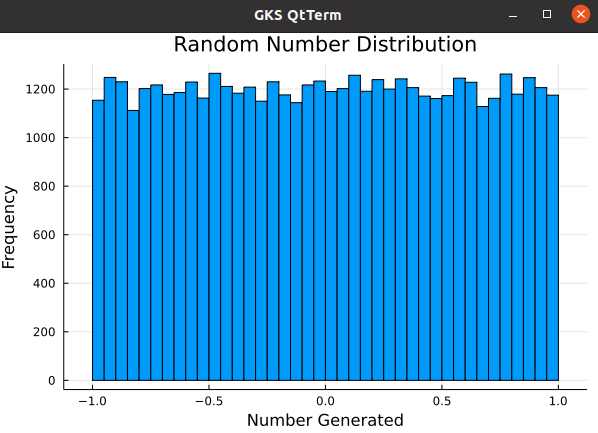
\includegraphics[width=0.6\columnwidth]{Figures/prac1_uniform_distribution.png}
\caption{Output of Plots.histogram(whiteNoiseArray)}
\label{fig:Julia_hist}
\end{figure}

\subsubsection{Timing Execution}
After confirming that your function works correctly use the TickTock package to compare the performance of the two approaches to generate white noise. In order to use the TickTok package run the command tick() to start the timer and the command tock() to stop the timer and output the time that has elapsed. Repeat the white noise generation process for varying sample sizes and consider add this to your report. 

\begin{lstlisting}
tick()
commands you wish to time
tock()
\end{lstlisting}

\subsubsection{Implementing Pearson's Correlation}
Implement the Pearson's correlation formula a new function call it \verb|corr()|. 

\subsubsection{Comparing Your Correlation Function to the Statistics Package's Correlation Function}
The \verb|cor| function in Statistics package performs a correlation operation. Compare your \verb|corr()| results to the Statistics.cor function. Run the following test:

\begin{enumerate}
    \item Using your output from the createWhiten(numberOfSeconds) function compare it correlation against itself using your correlation function and the Statistics.cor function.
    \item Compare the correlation between the two different approaches to generate white noise, using your correlation function and the Statistics.cor function.
\end{enumerate}


Do a table listing sample sizes vs. corr speed vs. Statistics.cor speed. Indicate the average speed-up, etc. in your report.

\subsubsection{Correlation of Shifted Signals}
For the last experiment, we want to compare signals shifted in time. Generate sin curves of varying frequency and sampling sizes (again sample sizes 100, 1000 and 10000 samples). Compare samples of the same sizes that are shifted in time, consider using the circshift(sineWave, 10), which will cause a shift of 10 samples.

For this step only use Statistics.cor to save time. In your report, discuss what you expect the correlation of the identical but shifted signals would be. Run tests to confirm / verify your hypothesis. Provide some screen shots plots of some of the signals you compared. It might be useful to use the Plots.scatter() function to generate these plots.


\subsection{Submission}
Hand in a report about 2-3 pages in length briefly describing your solutions for the tasks above. The format required is the IEEE conference format. Format your report as if it is an article (i.e. don’t follow the same chronology as the prac-sheet – format it as “Introduction – Method – Results and Discussion – Conclusion”). In the ``Method" section, theorise about what you expect and how you plan on testing said theory. In the ``Results" section, confirm that you obtained what you expected (or explain why you obtained something unexpected). Hint: You are trying to answer two questions: 1) ``Is my whitenoisen() function better suited to generated white noise, in comparison to the rand() equivalent?" 2) ``Is my corr() function better suited to run correlation tests, in comparison to the Statistics.cor equivalent?" and 2) ``Are my theories relating to the correlation of time-shifted sinusoids correct?" Provide key sections of code in your report. Marks will be awarded on elegance of your code and if your results have been portrayed in a logical way (i.e. tables and graphs).

\subsection{Marking}
\begin{table}[H]
\centering
\caption{Prac 1 Marking Guide}
\label{tbl:Prac1Marks}
\begin{tabular}{|l|l|r|}
\hline
\textbf{Aspect} & \textbf{Description} & \multicolumn{1}{l|}{\textbf{Mark Allocation}} \\ \hline
Report & Intro & 2 \\ \hline
 & Latex/Format & 1.5 \\ \hline
 & Headings etc & 1.5 \\ \hline
 & Captions & 1 \\ \hline
 & Discussion & 2 \\ \hline
createwhiten & Code & 4 \\ \hline
 & Histogram & 2 \\ \hline
 & Results & 3 \\ \hline
 & Conclusion and Explanation & 3 \\ \hline
Correlation & Code & 4 \\ \hline
 & Results & 2\\ \hline
 & Conclusion and Explanation & 2 \\ \hline
Shifted signals & Code & 4 \\ \hline
 & Plots & 3 \\ \hline
 & Results & 2 \\ \hline
 & Conclusion and Explanation & 3 \\ \hline

\textbf{TOTAL} &  & 40 \\ \hline
\end{tabular}
\end{table}
